\documentclass{ximera}
%% handout
%% space
%% newpage
%% numbers
%% nooutcomes

%% You can put user macros here
%% However, you cannot make new environments

\graphicspath{{./}{firstExample/}{secondExample/}}

\usepackage{tikz}
\usepackage{tkz-euclide}
\usetkzobj{all}
\pgfplotsset{compat=1.7} % prevents compile error.

\tikzstyle geometryDiagrams=[ultra thick,color=blue!50!black]
 %% we can turn off input when making a master document

\outcome{Encounter a scary example.}
\title{Nothing I Did Worked}
\author{Kirollos Masood}

\begin{document}
\begin{abstract}
In this activity, we will very brutally see the drawbacks and limitations of power series.
\end{abstract}
\maketitle

So far, we've seen that we can use power series to represent common functions. To be more explicit, we first start with a function we know. Then we write down the Taylor series expansion for the function around some center point. That's incredibly useful because we can approximate certain numbers (such as $e$) very easily by just including a few terms of the sum. We can also calculate very high order derivatives by looking at the coefficients, without excessively using the product rule.

Well what are the limitations? So far, the worst case scenario is that the power series diverges if we move too far away from the center point. But as long as we stay nearby, everything is fine. I'm sorry to say we've been sheltering you too much. The truth is that much more can go wrong. Let's take a look.

\begin{exercise}
	
	Let's introduce our first delinquent function.
	\begin{align*}
		f(x)= 
		\begin{cases}
		e^{-\frac{1}{x^2}}  &x \neq 0 \\
		0 &x=0
		\end{cases}
	\end{align*}
	
	Perhaps you feel uneasy whenever you see a piecewise-defined function. \emph{That's perfectly normal.} When we don't let $x=0$, the function seems as nice as can be. But what does happen at $x=0$? Let's take a look at a graph.
	
	\begin{image}
		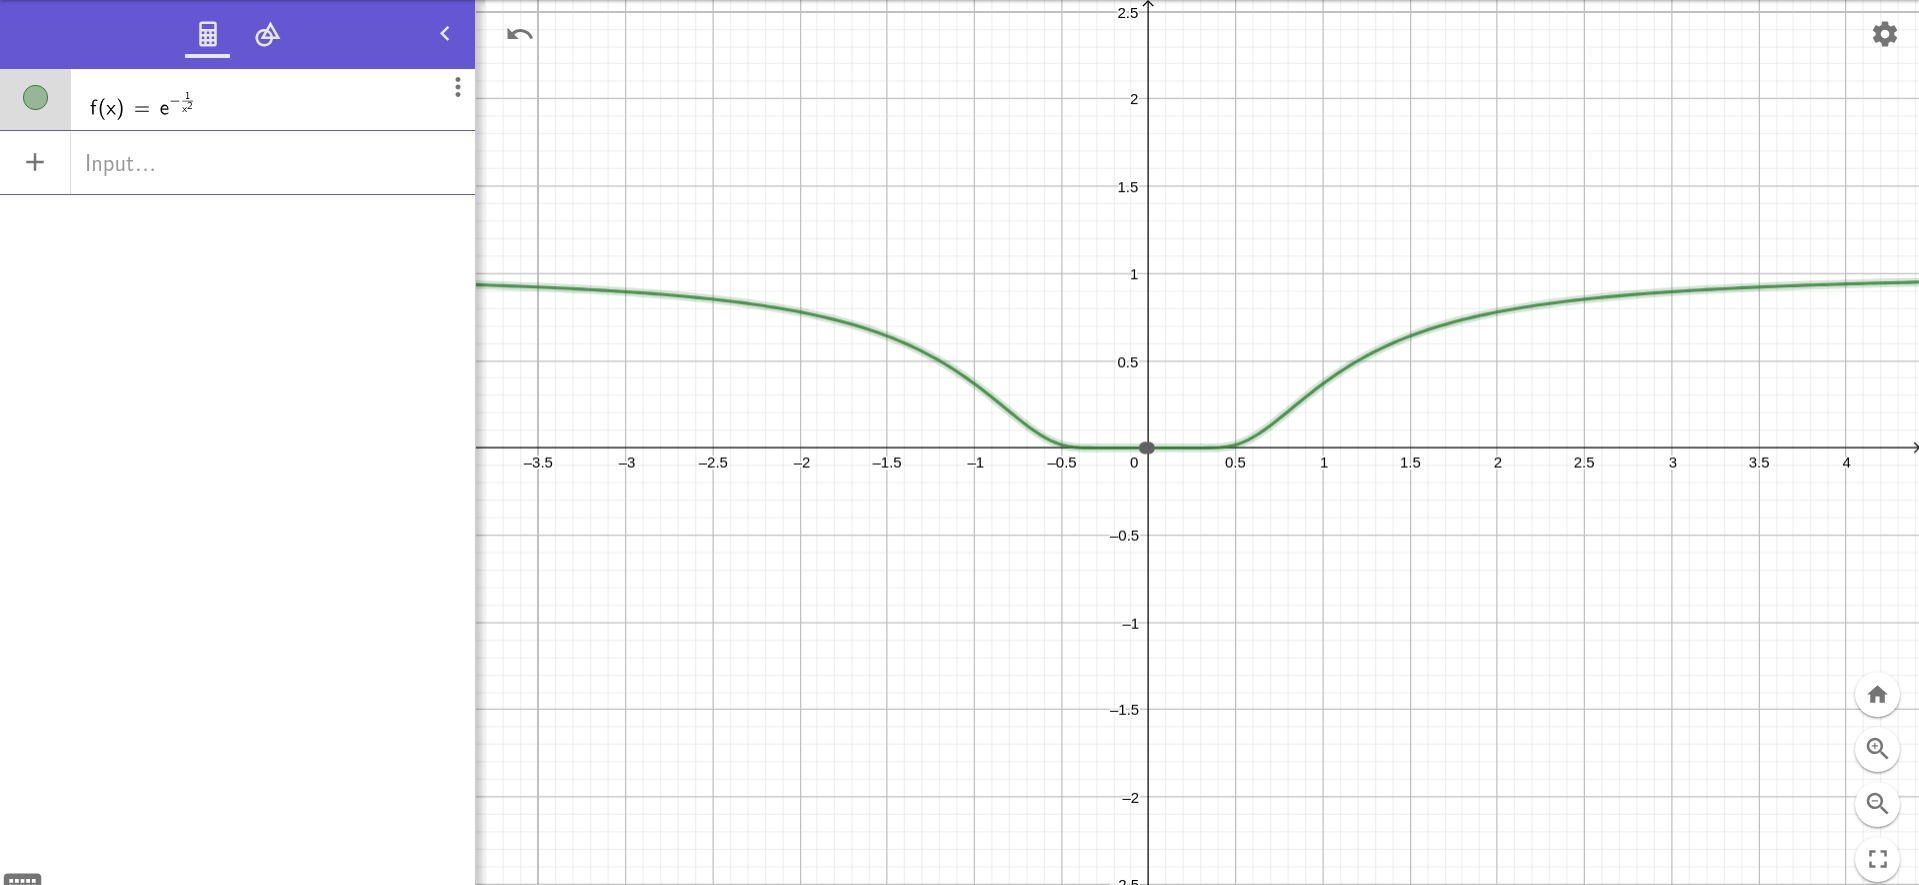
\includegraphics{graph.png}
	\end{image}
	
	We can visually see that this function is continuous at $x=0$. In fact, you can check that yourself without the graph by evaluating the appropriate limit. What's harder to swallow is that the function is differentiable too. Let's confirm this rigorously, which means we'll have to use the definition of the derivative. Don't panic! We'll walk through this together. Are you ready?
	\begin{multipleChoice}
		\choice[correct]{Sure. It's just a limit.}
	    \choice{No. It's been forever since I've done a derivative by hand. How did we even survive without rules of differentiation?}
	    \choice[correct]{Okay. I've calmed down. We can move on.}
	\end{multipleChoice}
	
	\begin{exercise}
		
		Since our function is even, it's enough to check the limit from the right. That'll make it easier since we'll want to use logarithms.
		\begin{align*}
			f'(0)= \lim_{h \to 0^+} \frac{f(0+h)-f(0)}{h} = \lim_{h \to 0^+} \frac{e^{-1/h^2}}{h} = \lim_{h \to 0^+} e^{-\frac{1}{h^2}}e^{-\ln(h)} = \lim_{h \to 0^+} e^{-\frac{h^2\ln(h)+1}{h^2}} = \answer[given]{0}
		\end{align*}
		
		\begin{exercise}
			And when $x \neq 0$, we can just use the chain rule with impunity. So we have the following.
			\begin{align*}
				f'(x)= 
				\begin{cases}
				\frac{2e^{-1/x^2}}{x^3}  &x \neq 0 \\
				0 &x=0
				\end{cases}
			\end{align*}
		\end{exercise}
		We see that this function is also continuous. But is it differentiable? Do you see where this is going? You can repeat this process as many times as you want. You can use the chain rule when $x$ is not $0$. And when $x=0$, you get $0$, no matter how many powers of $x$ end up appearing on the bottom. If you don't believe me, just try finding $f''(0)$. You'll soon learn that trust is a precious thing. Alright, so let's write down the Taylor series for $f(x)$ centered at $x=0$.
		\begin{align*}
			T(x) = \sum_{k=0}^{\infty} \frac{f^{(k)}(0)}{k!} x^k = 0
		\end{align*}
		Oh boy! We don't have to worry about the radius of convergence! This series converges for any value of $x\ldots$ to $0$. But where's our function!?
		
		We see that even though the Taylor series has all the right information about $f$ at $x=0$, it fails to be accurate anywhere else; we don't get back our function. No matter how close $x$ is to 0. Even though the radius of convergence is $\infty$. This is an example of a \dfn{non-analytic} function. 
		
		Non-analytic functions are those which cannot be recovered using a power series, for one reason or another. In this case, there was nothing wrong with the actual power series; our function just didn't match up with the end product. In some sense, $f$ just looked ``too flat'' at $x=0$. Our function simply wasn't nice enough, even though it was infinitely differentiable. Note that we call an infinitely differentiable function \dfn{smooth}.
		
		This is just one way a smooth function can fail to be analytic: its Taylor series expansion converges near the center but we just don't get our function back. Another way is that the resulting power series just doesn't converge no matter how close we are to the center (except of course exactly at $x=c$). We now move on to the next pathological suspect.
		\begin{align}
			g(x)=\sum_{k=0}^\infty e^{-k}\cos(k^2 x)
		\end{align}
		This function is defined for any value of $x$. To see this, you can simply test for absolute convergence. And while testing for absolute convergence, you can use just compare it to a geometric series. Oh and look! This function is already written as a series, so aren't we done? Well the issue is it isn't a \emph{power} series. The terms in the sums aren't powers of $x$. They are powers of $\cos(x)$. It is a very long and tedious process to show that the radius of convergence of the Taylor series centered at $x=0$ is $0$. Try it out yourself if you'd like, and feel free to come see me if you're stuck.
		
		So what do you think of non-analytic smooth functions?
		\begin{multipleChoice}
			\choice[correct]{I think they're cool!}
			\choice[correct]{I think they're atrocious.}
			\choice[correct]{I'm not sure I understand them.}
			\choice[correct]{I'm going to pretend they don't exist and hope I never run into one again.}
		\end{multipleChoice}
		
		
		
	\end{exercise}
	
\end{exercise}

\end{document}
